Our study compares individuals who experienced the Reggio Approach with those who experienced other Northern Italian early childhood programs, as well as some who undertook no program at all. In this section, we examine the similarities and differences across the available programs, both contemporaneously and historically. This section documents the Reggio Approach in addition to exploring the extent to which other programs offer features of the Reggio Approach at different points of time.

To increase our understanding of the evolution of early childhood programs in Reggio Emilia, Parma, and Padova, we administered a survey to current and former school administrators and educative coordinators in order to quantify pedagogical and administrative features of early childhood programs available during 1950-2010 \citep{CEHD_2016_Historical-Analysis}. See Appendix~\ref{sec:survey} for the survey. We further collected administrative data from historical archives in Reggio Emilia and Padova. We were unsuccessful in sourcing similar records from Parma \citep{Padova-Admin-Data_1964-2011,Reggio-Admin-data_1966-2006,Reggio-Annual-Journals_1994-2011}. Together, survey results and administrative data indicate that educational preschool was available to each cohort by various systems as listed in Table~\ref{tab:pre}. 

\begin{table}[H]
\centering
\caption{Availability of Preschool Programs by City and School Type}\label{tab:pre}
\begin{adjustbox}{width=\textwidth}
\begin{threeparttable}
	\begin{tabular}{l l c c c c c c c c c}
\toprule
\mc{1}{c}{Cohort} & \mc{1}{c}{Years} & \mc{3}{c}{Reggio Emilia} & \mc{3}{c}{Parma} & \mc{3}{c}{Padova} \\
& & Municipal & Catholic & State & Municipal & Catholic & State & Municipal & Catholic & State \\
\midrule
Adults 50s & 1957-1965 & & \checkmark & & & \checkmark & & & \checkmark & \\
Adults 40s & 1972-1976 & \checkmark & \checkmark & & & \checkmark & & & \checkmark & \\
Adults 30s & 1983-1987 & \checkmark & \checkmark & \checkmark & \checkmark & \checkmark & \checkmark & \checkmark & \checkmark & \checkmark \\
Adolescents & 1994-2000 & \checkmark & \checkmark & \checkmark & \checkmark & \checkmark & \checkmark & \checkmark & \checkmark & \checkmark \\
Children & 2009-2014 & \checkmark & \checkmark & \checkmark & \checkmark & \checkmark & \checkmark & \checkmark & \checkmark & \checkmark \\
\bottomrule
\end{tabular}

% Caption:
% Note: This table indicates the types of educational preschool systems (defined as programs with 4 or more sites) available to parents in each city during the years each cohort was eligible for a 3-6 year old program. 
\begin{tablenotes}
Note: This table indicates the provision by system of educational preschool systems (defined as programs with 4 or more sites) available in each city during the years each cohort was eligible to attend a 3-6 year old program. 
\end{tablenotes}
\end{threeparttable}
\end{adjustbox}
\end{table}

The survey was designed to explore the extent to which the key administrative and pedagogical components of the Reggio Approach were present in each city's state, religious, and municipal systems at different points of time. The components included in the survey were identified by published program descriptions and confirmed by scholars of the Reggio Approach and early childhood programs in Northern Italy.\footnote{See \citet{Edwards-etal-eds_1998_Hundred-Languages} and \citet{Corsaro_2008_Policy-Practice}.} The list of components includes various aspects of administrative program operations such as staffing, supervision, enrollment, and funding. It also considers pedagogy and educational practices for children's learning and parental engagement. Respondents were asked to indicate whether central features of Reggio were present in their systems during different decades. Additional questions were included to understand a) the extent of variation between municipal programs and private providers contracted by the municipality; b) the extent of site-level variation within systems; c) the perceived variation between similar systems in other cities; d) the sources of program funding, and e) the services available for immigrant families.\footnote{For a more detailed summary of the items and the responses, see Appendix~\ref{sec:survey}.} Table~\ref{tab:respondents} identifies the school systems in each city that completed our survey.

\begin{table}[H]
\centering
\caption{Survey Respondents by City and School Type}\label{tab:respondents}
\begin{threeparttable}
	\begin{tabular}{lccc}
\toprule
City & Municipal & State & Religious \\
\midrule
Reggio Emilia & \checkmark & \checkmark & \\
Parma		& \checkmark & & \\
Padova & \checkmark & \checkmark & \checkmark \\
\bottomrule
\end{tabular}
\begin{tablenotes}
\footnotesize Note: This table indicates the systems represented by survey respondents. These individuals include current and former administrators and educational coordinators. One survey was administered for each system noted. Answers reflect the input of multiple people associated with the system. Responses were provided by religious systems in Reggio Emilia and Parma, however, they do not include historical data prior to 2000.
\end{tablenotes}
\end{threeparttable}
\end{table}

\textbf{[JJH: Flatten table.][Edited]}

Results from the survey indicate that early childhood education systems within Reggio Emilia, as well as in Parma and Padova, share a number of similar characteristics. These include features of program administration, various pedagogical methods, and practices for at-risk children and families. The general trend shows that programming and practices endorsed by the municipality of Reggio Emilia are present in other early childhood systems, albeit to different degrees and at different times. These results mildly support a spillover story of Reggio Approach features into other early childhood programs given that treatment effects are found only for the oldest cohorts. The general trend is also consistent with the explanation that common influences were operating at the onset of these programs. \textbf{[JJH: How can a survey reveal spillovers or not? Team: We have adjusted the text to reflect ]} We do acknowledge that the small sample of survey respondents may be too limited to ensure reliable results.

We compare the different programs in Figures~\ref{fig:agg-admin} and~\ref{fig:agg-ped}. A more detailed description is provided in the section that follows. Using survey results, we calculate the number of administrative and pedagogical components that each program shared with the Reggio Approach by school type, city, and year. We examine 14 administrative components and 16 pedagogical components (not all of the pedagogical components were present in the Reggio Approach). Over time, many of the programs implemented more and more of the pedagogical and administrative practices endorsed by the Reggio Approach. This is especially true for Parma's municipal program, and true to a somewhat lesser extent for Padova's municipal program. The other systems did not adopt as many pedagogical components as they did administrative ones. Even though the Reggio Approach remains distinctive when considering the sum of its elements, many of the alternative schools evolved to include a substantial portion of the elements in Reggio Emilia's municipal system.

\textbf{[JJH: Please break out the pedagogical components --- summing conceptually different items is a meaningless exercise.]}

\begin{figure}[H]
\begin{center}
\begin{subfigure}[b]{0.49\textwidth}
	\caption{Number of Administrative Characteristics in Common with the Reggio Approach}\label{fig:agg-admin}
	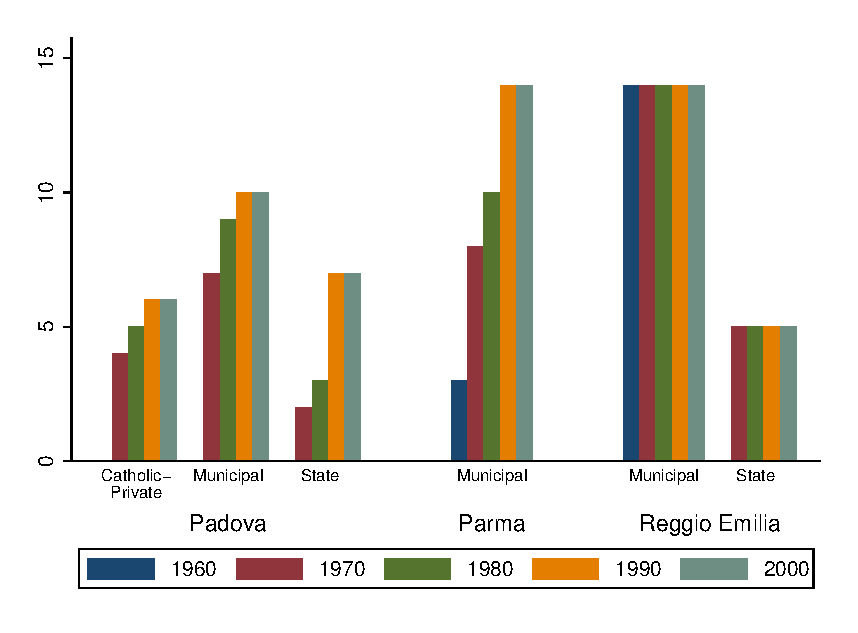
\includegraphics[width=\textwidth]{../../output/aggregateAdministrative.eps}
\end{subfigure}%
~
\begin{subfigure}[b]{0.49\textwidth}
	\caption{Number of Pedagogical Characteristics in Common with the Reggio Approach}\label{fig:agg-ped}
	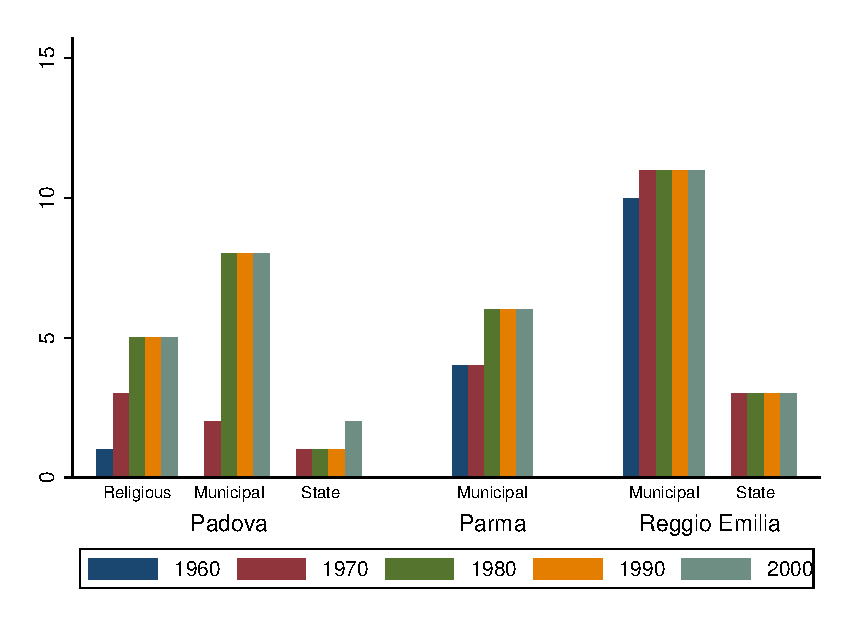
\includegraphics[width=\textwidth]{../../output/aggregatePedagogical.eps}
\end{subfigure}%
\end{center}
\raggedright \footnotesize Note: These graphs show the number of administrative and pedagogical components that each program has in common with the Reggio Approach. We consider 14 administrative components and 16 pedagogical components. Some of the pedagogical components were not present in the Reggio Approach.
\end{figure}

\textbf{[JJH: Can we put in color?] [Typist: Professor, these are currently in color. We will print you a color version tonight.]}

\textbf{[JJH: Earlier we say we have no historical data on Parma -- now suddenly we do. Which is correct? Sylvi: Parma's municipal system DID respond to our survey as indicated in Table 1. We could not, however, retrieve important administrative data from Parma's municipal archives. We better clarify this distinction in the second paragraph of this section.]}

%\footnote{See Appendix~\ref{} for more extensive discussion of the survey results.}

\subsection{Municipal Schools in Reggio Emilia - The Reggio Approach}

Of the municipal systems in Reggio Emilia, Parma, and Padova, the Reggio Approach is notable for creative programming \textbf{[JJH: Innovative how? Please cut the bombast.][Edited to be more precise.]}, investment in staffing, and broad provision of early childhood services. Of the three, it was the earliest municipal system to evolve and it consistently funded and managed the largest number of municipal infant-toddler and preschool sites.\footnote{Similar to Parma and Padova, Reggio Emilia contracts with local private providers and cooperatives to offer infant-toddler and preschool slots according to municipal regulations. These ``affiliated'' programs may not follow the Reggio Approach nor the municipal approaches in Parma and Padova. Accordingly, we consider this a separate sample during analysis.} 

In 1963, Reggio Emilia constructed its first preschool for children aged 3-6 years; by 1975, the municipality offered 19 preschools \citep{Hohnerlein_2009_Paradox-Public-Preschools}. In 1965, the municipality legislated funding for infant-toddler centers for children aged 3 to 36 months. The first site opened in 1971, and ten more were added by 1979 \citep{Cagliari-etal-eds_2016_BOOK_Loris-Malaguzzi}. Reggio Emilia thus preceded Italy's key educational reforms of 1968 and 1971 legislating free state preschools and local provision of infant-toddler childcare. \textbf{[JJH: Can we say that Reggio actually influenced reforms? Sylvi: I don't recommend saying this because Hohnerlein, a non-Reggio scholar, credits Bruno Ciari in Bologna for influencing state reforms for public preschool. In addition, the 2001 OECD report, authored by FPGC scholar Rebecca New, states that Malaguzzi's influence was pedagogical (i.e., creativity as a vehicle for learning, pedagogistas, arts educators). Reggio Emilia hosted 2 large conferences for educators in the early 1970s, along with other local cities, to disseminate these new approaches throughout Italy. Shall we state this?]}

The Reggio Approach is a form of progressive early childhood education shaped by Loris Malaguzzi, a psychologist and educator influenced by Dewey's model of progressive education, Vygotsky, and psychological theories of Piaget, Erikson, Bruner, Bronfenbrenner, Kagan, and Gardner \citep{Rinaldi_2006_ReggioEmilia_BOOK,Cagliari-etal-eds_2016_BOOK_Loris-Malaguzzi} \textbf{[JJH: Do we know this? Please give me a citation. Talk is cheap and people rationalize what they did, see e.g., the Perry teacher survey. Did Reggio evolve? Gardner could not have had an effect. Sylvi: According to the 2016 Malaguzzi book, the features we reference in our survey were all in place by 1972. The book does cite these influences on Malaguzzi and the Reggio Approach.]} In 1972, under Malaguzzi's direction, the municipality officially adopted Regulations for Municipal Schools that clarify community values for children, roles of parents and community members in school management, administrative operations, enrollment priorities, and environmental features of preschools and infant-toddler centers \citep{Giaroni_1972_Regulations-Municipal-EC-Schools}.

The engagement of families and the community is embedded in the Reggio Approach. Parents and community members participate in school management to shape policies. Parents volunteer in classrooms and community members host field trips in the city \citep{CEHD_2016_Historical-Analysis,Cagliari-etal-eds_2016_BOOK_Loris-Malaguzzi}. To accommodate working parents, preschools and infant-toddler centers are open five full-time days per week from September through June \citep{Giudici-Nicolosi_2014_Reggio-Approach}. Some sites offer programming in July and extended day options are available at a majority of sites throughout the school year. To support all children in the community, Reggio Approach schools prioritize admission for children with disabilities, providing occupational, physical, and speech therapy as needed \citep{Edwards-etal-eds_1998_Hundred-Languages,Giaroni_1972_Regulations-Municipal-EC-Schools}

In preschools, incoming 3-year old cohorts form a homogenous classroom of about 25-30 children. Each cohort, according to municipal guidelines, are assigned two full-time co-teachers (teacher-pupil ratios are 1:12-13). \textbf{[JJH: Seems high! Sylvi: Compared to the US, it does seem high. Compared to Italy's state and religious schools, it was lower until the 2000s. We discuss this in the State subsection.]} At least 1 of the 2 teachers remains with each cohort for three consecutive years, offering extended time for continuity of care and strong teacher-family engagement. Each preschool site is also staffed by a full-time atelierista, an instructor with a background in visual arts, who helps teachers develop creative learning activities. On a biweekly basis, a pedagogista with a minimum bachelor's degree in psychology or pedagogy \textbf{[JJH: Post-BA? Be specific! Sylvi: Confirmed.]} supports the professional development for the educational staff of approximately 4-5 municipal preschools. Auxiliary site staff, such as cooks and janitors, are considered members of the educational team and participate in the biweekly trainings.\footnote{The Reggio Approach encouraged staffing of male educators in preschools from its inception. This policy conflicted with state law until 1978 \citep{Hohnerlein_2015_Development-and-Diffusion}.}

Reggio Approach environments reflect a light-filled, open interior design, furnished with natural materials and a garden. Each preschool is equipped with an atelier, or dedicated studio laboratory, where children and educators collaborate on creative instructional activities. In-house kitchens are surrounded by glass walls, to include children in the meal preparation process, and is used daily for preparing meals \citep{Rinaldi_2006_ReggioEmilia_BOOK,Vecchi_2010_ReggioEmilia_BOOK}. 

In Reggio Approach pedagogy, there is no institutionally-prescribed content knowledge that educators convey to children to achieve the goal of ``school readiness,'' or any other such goal. Instead, curriculum is viewed as an ongoing, collaborative project between educators, children and families. Learning goals are achieved through creative long-term projects with flexible timelines. Adults and children are jointly viewed as researchers and co-creators of knowledge. For example, adults and children collaborate to define a question or topic. Learning is then pursued following a scientific process: theories are shared, tested, and revised through socratic questions and dialogue. \textbf{[JJH: Reggio's curriculum is more method than content (in contrast to state, religious, and the other municipal programs which emphasize content). But this is not shared by other schools? How do we know? Sylvi: We asked two questions about this in our survey, and the scholar who collected survey data in Padova on our behalf confirmed this.]} Teachers observe children's development, listen, interact with children through questions and dialogue, and provide scaffolding to extend learning. Children demonstrate their emerging knowledge through expressive art forms, with aid from the atelierista. Teachers organize each child's documented work in a portfolio that is shared with children and parents over the year to observe the child's development \citep{Rinaldi_2006_ReggioEmilia_BOOK,Giudici-Nicolosi_2014_Reggio-Approach}.

\subsection{Municipal Schools in Parma and Padova}

\textbf{[JJH: This section is very weak and hurts the paper. Sylvi: This section has been revised.]}

Survey results, reports, and interviews indicate that the municipal early childhood systems in Parma and Padova both grow more similar over time to the Reggio Approach. From their inception, the three municipal systems share many features including a strong emphasis on the provision of high quality programming for infant-toddler centers \citep{Ghedini_2001_Ital-Natl-Policy}. From the 1970s forward, each city invested in staffing municipal schools for 8 hours daily, extended hours for working families, and prioritized enrollment for low-income families. Each city emphasized family participation in school management. From the 1980s forward, all three municipal school environments featured an atelier, in-house kitchens, open spaces, and the use of natural lighting and materials. Furthermore, educational approaches were influenced by the same academic theories of psychology and education. From the 1990s forward, all cities prioritized enrollment for children with disabilities \footnote{In Padova, prioritized enrollment for children with disabilities began in the 1970s.} and included project-based learning as a teaching method.

Of the two cities, Parma's municipal system is more similar in policy and administrational operations to that of Reggio Emilia, sharing the same approach from the 1990s. For example, Parma reports that administrative operations, weekly scheduled hours to engage families, and professional development for teachers began to appear in the mid-late 1970s.\footnote{In Padova, professional development for municipal early childhood staff began in the mid-1980s \citep{Becchi-Ferrari_1990_Pub-Inf-Centres-Italy}.} From the mid-late 1980s, Parma focused on improving management of infant-toddler centers to support the varying needs of working parents. 

From a pedagogical perspective, however, survey results suggest that municipal early childhood programming in Padova is more consistently similar  to the Reggio Approach. In Padova, teachers began to document children's learning in the 1970s. By the 1980s, fine arts specialists were hired to support creative learning activities. 
\textbf{[JJH: It is only in the 2000s. What is the evidence? Sylvi: We have added content from earlier decades.]} 

Where the Reggio Approach and the municipal systems in Parma and Padova differ is in the application of psychological theories to pedagogical methods. In both Parma and Padova's municipal systems, classrooms are heterogenous in age and religious instruction is provided. In contrast to the Reggio Approach where content learning is secondary to creative expression, daily activities in the municipal preschools of Parma and Padova follow a program to guide children in learning specific concepts such as communication, culture, order, measure, space, time, nature, self, and other. In Padova, cognitive development is emphasized, teaching includes direct-instruction, and children complete worksheets as a learning activity \citep{CEHD_2016_Historical-Analysis}. 

Overall, relative to Reggio Emilia, investment in municipal early childhood programs for ages 0-6 by Parma and Padova occurred approximately 10 years and 15 years later, respectively. In considering selection into different systems by families in each city, we note that Parma and Padova each provided fewer municipal infant-toddler centers and preschools from the 1960s forward. We further note that enrollment is highest in the municipal preschools of Reggio Emilia and Parma, whereas in Padova, it is secondary to enrollment in religious preschools \citep{Padova-Admin-Data_1964-2011,Reggio-Admin-data_1966-2006,Reggio-Annual-Journals_1994-2011}. 

The evidence presented supports the finding of more significant outcomes for the Age 40 cohort than the Age 30 cohort, and fewer differences for Adolescents and Children in comparisons between municipal programs. For additional information, see (see Appendix Tables~\ref{tab:programoperation} to \ref{tab:environ-features}). 
%\textbf{[JJH: Such as? Sylvi: The program concepts are intentionally vague in order to be actualized at the individual school-level, similar to Head Start. (In contrast, in Reggio, chosen concepts are not pre-determined but follow the child's lead.)]} \textbf{[JJH: Why inconsistent?] [Sylvi: Apologies, I'm unsure what inconsistency you refer to.] [JJH: This has to stop. It's obvious what I said. Knowing order, space, time, etc. is not consistent with Reggio. There is no head to head comparison. It looks like Sylvi swallowed Reggio propaganda hook, line, and sinker.]}.

\subsection{State Preschools}

Over time and across cities, each cohort in our sample had access to differential numbers to state preschools. Further those who enrolled in state programs experienced varying early childhood curricula and administrative practices.

State preschools are mandated by the 1968 Law 444 regarding the provision and funding of a system of public preschools. Law 444 dictated state teachers be female, less than 35 years old, and hold a vocational high school diploma from a 3-year school. In state programs, parents pay only for meals and transportation. \textbf{[JJH: Discuss features of the 1968 literature. Sylvi: This is added.]} Law 444 resulted in disparate numbers of state preschools in Reggio Emilia, Parma, and Padova for each of the cohorts in our evaluation by mandating that state preschools only be funded where local demand was not already met by existing non-state systems such as municipal and religious schools \citep{Hohnerlein_2009_Paradox-Public-Preschools}. Historical records indicate that state preschools first appeared in Reggio Emilia and Padova between 1973-1975 \citep{Padova-Admin-Data_1964-2011,Reggio-Admin-data_1966-2006,Reggio-Annual-Journals_1994-2011}. In contrast to other areas of Italy where the state is currently the largest provider of preschool education, enrollment in Reggio Emilia, Parma, and Padova's state preschools has historically lagged behind municipal and religious programs. Although the state does not offer infant-toddler childcare, it regulates and subsidizes these programs through regional governments per 1971 Law 1044.
\textbf{[JJH: What is municipal and what is municipal preschool?]}

Reports suggest that periodic reforms to state laws and revisions to guidelines for state schools (Orientamenti) were historically influenced by municipal programs from the region of Emilia Romagna, including Reggio Emilia, Milan, and Pistoia \citep{OECD_2001_Italy-Country-Note}. Improvements to Orientamenti, along with revised mandates for lower teacher-child ratios and higher qualifications for teacher education, are proposed as key quality indicators associated with diminishing disparities in state and non-state programs by the end of the 20th century \citep{Hohnerlein_2015_Development-and-Diffusion}. For example, child-teacher ratios were very high for the three adult cohorts ranging from 27 to 36 children aged 3-5 years per teacher. Attendees of state preschools in the adolescent cohort experienced a 1:17 teacher-child ratio. For the child cohort, teacher-child ratios in state preschools was equivalent to that of the Reggio Approach \citep{Hohnerlein_2015_Development-and-Diffusion}.

Survey results indicate that the administration of state preschools are different from the Reggio Approach and from municipal programs in Parma and Padova. For example, state preschools do not offer extended hours to working families. At 30 hours per week, state teachers work 6 hours less than their municipal counterparts. Due to reduced hours, however, children in state preschool classrooms spend more time with only 1 teacher than do children in municipal preschools. State preschools do not hire an expert in the creative arts and do not set aside time for teachers to engage families (see Appendix Table \ref{tab:programoperation}). 

Survey results further suggest that administrative operations for state preschools in Padova are similar to state preschools in Reggio Emilia, with two interesting exceptions: First, in Padova, parents must pay for extras such as field trips, whereas in Reggio Emilia, field trips for children in state preschools are funded by the municipality. Second, Padova reports staffing educational coordinators to provide professional development for state teachers from the 1990s forward. 

Overall, pedagogy in state preschools supports children's learning differently than in the Reggio Approach. Teaching in state preschools evolved over time; the most notable revision to guidelines occurred in 1991 when social, emotional, and cognitive development were first emphasized. Similar to municipal schools in Parma and Padova, survey results further indicate that teaching in state preschools is influenced by different academic theories, religious teaching is provided, and daily activities follow a program to guide children in learning of specific concepts (see Appendix Tables~\ref{tab:programoperation} to \ref{tab:environ-features}).  

Our study evaluated whether these additional features of Reggio have any benefits. They appear not to. \textbf{[Team: We propose the following revision: Our study evaluated whether these features of the Reggio Approach were effective in benefitting individuals sufficiently to result in significant improvement in outcomes relative to individuals who did not receive the Reggio Approach. They appear not to.]}

\subsection{Religious Preschools}

The Catholic Church is the oldest early childhood provider in Italy, offering both religious training and charitable social services for disadvantaged children since the 19th century \citep{OECD_2001_Italy-Country-Note}. All five cohorts in our evaluation had access to religious programming for ages 3-6 years. Until the 1990s, religious schools in Reggio Emilia, Parma, and Padova did not offer educational infant-toddler programs. The Adolescent cohort had access to a several months of transitional programming for children over 24 months of age in each of the three cities. The Child cohort had access to infant-toddler programs from the age of 12 months \citep{Malizia-Cicatelli_2011_BOOK_Catholic-School,CEHD_2016_Historical-Analysis}.

Administratively, local federations of religious schools began to assemble throughout Italy in the mid-1970s. Religious preschools within the cities of Reggio Emilia, Parma, and Padova could join a city-level local federation that supported administrative operations. \textbf{[JJH: Churches? What's a site? Church? Sylvi: Correct. JJH: What is the content of the program?]} In contrast to the Reggio Approach, however, religious schools do not implement a unified model of religious preschool education; thus there is no single approach that is shared by all religious programs within each city or between cities. 

Following a 1997 policy, however, that enabled state funding for non-state programs (i.e., municipal and religious) meeting national guidelines for early childhood, the Catholic Church undertook significant efforts to quantify and achieve equitable program quality \citep{Malizia-Cicatelli_2011_BOOK_Catholic-School}. From this date forward, educational programming and policies in equitable religious preschools reflected state laws and guidelines. For example, after 2000, religious educators were replaced with secular teachers trained in higher institutions and teacher-child ratios were greatly reduced to reflect national standards. Children experienced educational programming that reflected, like state preschools, the influence of municipal systems in Emilia Romagna, including Reggio Emilia \citep{Hohnerlein_2009_Paradox-Public-Preschools,OECD_2001_Italy-Country-Note}. Families of the Child cohort who enrolled in equitable religious programs were eligible for subsidized tuition on a sliding-scale basis; prior to this date, tuition and fees for religious preschool in all three cities was more expensive than the cost of municipal and state programs.

Survey results for religious preschools are only available for Padova. Evidence suggests that religious preschools in Padova share the following practices with the Reggio Approach: from the 1970s, weekly time was set aside for teachers to engage families and the same teacher remained with a cohort of children. Parental boards are actively engaged in the school culture from the 1970s (see Appendix Table \ref{tab:programoperation}). From 1980s, teachers documented children's work and school environments included an atelier, or dedicated room where children worked together (see Appendix Table \ref{tab:environ-features}). From the 1990s, Padova's religious schools prioritized enrollment for children with disabilities. 

Unlike the Reggio Approach, Padova's religious preschools provide religious teaching and follow a daily program to guide children in learning specific concepts (see Appendix Table \ref{tab:educ-program}). Further, they do not prioritize the enrollment of children from economically disadvantaged families (see Appendix Table \ref{tab:administrative-atrisk}). This appears to have no effects for the measures we study.

\subsection{Summary}

On many key features, Reggio is no longer unique, if it ever was. \textbf{[Team: We recommend dropping "if it ever was".]} The evidence summarized here supports the empirical work, which we report next.

